\chapter{Differential Equation Solvers}
\label{Cha:DESolvers}
A differential equation solver allows one to compute the solution of a
differential equation numerically. A numerical method will result in a
discretized approximation to the solution. Although there are methods that can
solve differential equations exactly, they are not in practice useful since
there are many systems that don't have an analytic solution that
would require case by case symbolic manipulation. Numerical methods are more
easily applied.

The differential equations encountered in this thesis are all ordinary
differential equations (ODE), as opposed to partial differential equations. The
\textit{order} of a differential equation is the number of the highest
derivative in the equation. For example
\begin{equation}
    \label{Eqn:2ndODESpec}
	\mathbf{\ddot{x}}(t) + 3\mathbf{\dot{x}}(t) + 2\mathbf{x}(t) = 0
\end{equation}
is a differential equation of order 2. To \textit{satisfy or solve} the above
equation means finding a function for $\mathbf{x}$ that, when plugged into the
equation, results in $0$ which is the RHS. A more general form of a 2nd order ODE can
be written as follows
\begin{equation}
    \label{Eqn:2ndODE1}
    \mathbf{\ddot{x}}(t) = \mathbf{f}(\mathbf{\dot{x}}, \mathbf{x}, t)  
\end{equation}
Matching the general form with the specific example given above results in 
\begin{equation}
    \label{Eqn:2ndODESpec1}
    \mathbf{\ddot{x}}(t) = -3\mathbf{\dot{x}}(t) -2\mathbf{x}(t)
\end{equation}
There are many solutions for \ref{Eqn:2ndODESpec}.
For example given the following function
\begin{equation}
    \label{Eqn:Example}
    \dot{f}(t) = t^2
\end{equation}
then
\begin{equation}
    \label{Eqn:Example1}
    f(t) = \frac{t^3}{2} + C
\end{equation}
represents a solution.
In order to uniquely determine a solution more information about $f$ at a
certain time $t_0$ is required. If this information is available
\[
    f(t_0) = a
\] 
then $C$ can be evaluated and a unique solution found. Likewise, when it comes
to solving a differential equation, a set of \textit{initial conditions} are
required, similar to the one for $f$ given above. For \ref{Eqn:2ndODE1} (and hence
\ref{Eqn:2ndODESpec}) a valid initial condition is the pair
\begin{eqnarray*}
    \dot{\mathbf{x}}(t_0) = \dot{\mathbf{x}}_0\\
    \mathbf{x}(t_0) = \mathbf{x}_0
\end{eqnarray*}
Knowing these values a unique solution can be found.
An example of an invalid initial condition is
\begin{eqnarray*}
    \mathbf{x}(t_0) = \mathbf{a}\\
    \mathbf{x}(t_0) = \mathbf{b}
\end{eqnarray*}
Another example of a condition placed on the system is 
\begin{eqnarray*}
    \mathbf{x}(t_0) = \mathbf{a}\\
    \mathbf{x}(t_1) = \mathbf{b}
\end{eqnarray*}
This gives the positions of the particles at different times and is known as a
two point boundary condition. These require elaborate solution methods that are
not dealt with in this thesis.

The differential equations in this thesis are all ODEs of order
1 or 2, however, the algorithms discussed can be applied to higher order ODEs.
In fact, a higher order ODE can be reduced to a system of 1st order ODEs
\cite[pg 208]{NagleSaff}. This is important because the numerical
algorithms used work on 1st order ODE's.

\section{Euler's Method}
\label{sec:EulerMethod}
Euler's method is a differential equation solver that one may have coded before
and not known it by it's formal name. An intuitive understanding of how it works
can be gained by recalling the high school maths days when a formula for the
position of a particle was given as speed (assuming that the speed is constant)
multiplied by the elapsed time.
\[
    x(t) = speed * time 
\]
Knowing this formula it was easy to implement an algorithm to animate a
particles motion.
\begin{verbatim}
    while (....)     
        dt = current_time - last_time
        x = old_x + speed * dt        
\end{verbatim}
The algorithm above will build up an approximation for x using the
derivative of x, which is speed in this case. 

Euler's method works be evaluating the gradient of a function, $\dot{x}(t)$, at
a point and then travelling along that gradient a distance, governed by the step
size, before evaluating the gradient again.
\begin{equation}
\label{euler}
	\mathbf{x}(t_0+\Delta t) \approx \mathbf{x}(t_0) + 
		\Delta{t}\mathbf{\dot{x}}(t_0)
\end{equation}


Decreasing the step size improves the accuracy of the approximation. However for
the Euler method to achieve the same level of accuracy as other methods, like
the 4th order Runga-Kutta, the step size has to be much smaller than the step
size used for the other method. The Euler method is only first order accurate.
This means that if the function in question is non-linear (i.e. the 2nd or
greater order derivative exists) then the approximation becomes inaccurate. For
example if the speed of the particle is not constant, the particle is
accelerating and the 2nd derivative of position exists, then using Euler's method
will yield an inaccurate solution.  
    
In order to see that the Euler solver is 1st order accurate recall that the
Taylor series lets one write a function in terms of its derivative at a
specified point.
\begin{equation}
	\label{taylor}
	\mathbf{x}(t) = \mathbf{x}(t_0) + \mathbf{\dot{x}}(t_0)(t - t_0) +
		\frac{\mathbf{\ddot{x}}(t_0)}{2!}(t - t_0)^2 + . . .
\end{equation}
Since we want to know the value at $t_0+\Delta t$ we substitute it in
$t$ in the above equation and get
\begin{equation}
	\label{taylordt}
	\mathbf{x}(t_0 + \Delta t) = \mathbf{x}(t_0) + 
		\mathbf{\dot{x}}(t_0)\Delta t + 
		\frac{\mathbf{\ddot{x}}(t_0)}{2!}\Delta t^2 + . . .
\end{equation}
As you can see the first two terms of the Taylor series are the terms in the
Euler method. This means that the error is the the difference between
\ref{euler} and \ref{taylordt}. The dominant term in the error series is  
\[
    \frac{\mathbf{\ddot{x}}(t_0)}{2!}\Delta t^2
\]

The Euler solver is also unstable. It diverges when using large time steps. Of
course, by making the time steps smaller one can reduce this divergence, however
the cost comes in the number of steps needed to achieve the approximation. In
physically based animation the goal is to make the simulation look good. The
accuracy of the simulation, although important, is in practice sacrificed in
favour of looking good. A first order method that has a tendancy to be unstable
won't satisfy either of these goals.

\begin{figure}
	\begin{center}
    		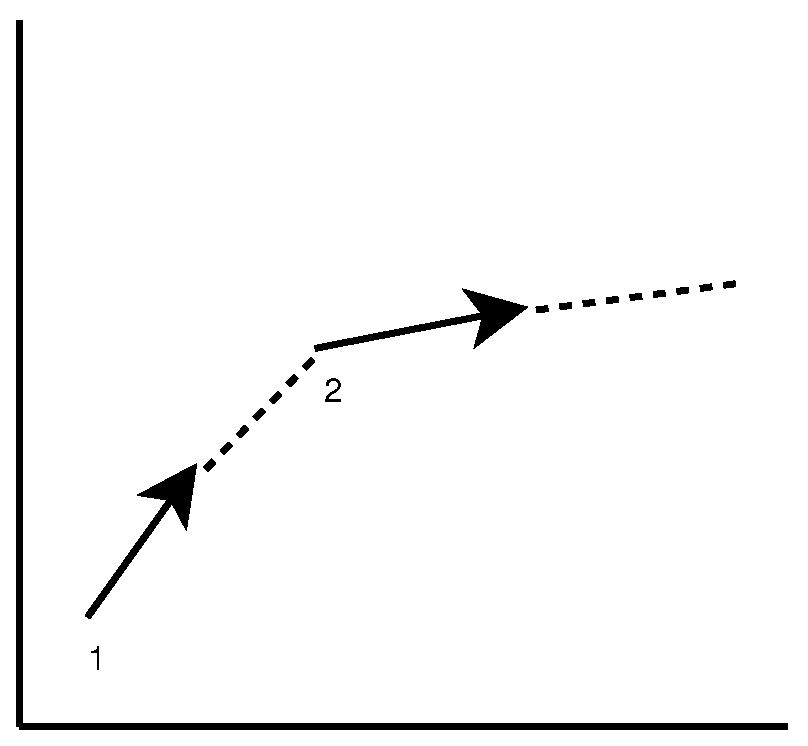
\includegraphics[height=0.25\textheight]{Euler}
	\end{center}
    \caption{\label{Fig:Euler}Euler's method. The diagram shows Euler's
    method working out the derivative at 1 and using that gradient to
    approximate that value of the function until the next point is reached. Then
    the derivative is evaluated again. This figure is based on the one shown in
    Numerical Recipes \cite{NumRecipes}.}
\end{figure}

\section{Midpoint Method}
The midpoint method is a 2nd order method. It works by computing the gradient at
the start, $x_0$, moving half a step size ($\frac{\Delta t}{2}$) in this
direction, then re-evaluating the gradient at the midpoint. A full step ($\Delta
t$) from $x(t_0)$ to $x(t_0 + \Delta t)$ is taken in the new direction.

\begin{eqnarray}
    \mathbf{k}_1 = \frac{1}{2}\Delta t \dot{\mathbf{x}}(t_0)\\
    \mathbf{k}_2 = \mathbf{x}(t_0) + \Delta t \mathbf{k}_1
\end{eqnarray}

A mathematical verification of that it is a 2nd order method can be found in
\cite{Otte, NagleSaff}
\section{Runge-Kutta 4}
\label{sec:RungeKutta4}
The 4th order Runge Kutta was the prefered algorithm for numerical solving
differential equations because it is more stable and accurate than Euler's
method. The algorithm is well documented in many texts \cite{Eberly,NagleSaff}
and is included below
\begin{eqnarray*}
    \mathbf{k}_1 &=& h\mathbf{F}(t_i,\mathbf{x}_i) \\
    \mathbf{k}_2 &=& h\mathbf{F}(t_i + \frac{h}{2},\mathbf{x}_i + h\frac{\mathbf{k}_1}{2})\\ 
    \mathbf{k}_3 &=& h\mathbf{F}(t_i + \frac{h}{2},\mathbf{x}_i + h\frac{\mathbf{k}_2}{2}) \\
    \mathbf{k}_4 &=& h\mathbf{F}(t_i + h, \mathbf{x}_i + h\mathbf{k}_3)\\
    \mathbf{x}_{i+1} &=& \mathbf{x}_i + \frac{1}{6}(\mathbf{k}_1 + 2\mathbf{k}_2
        + 2\mathbf{k}_3 + \mathbf{k}_4)\\
    t_{i+1} &=& t_i + h
\end{eqnarray*}
$\mathbf{F}$ is a function that returns the derivative at the given point and
time. In other words $\mathbf{F}(x,t)=\dot{x}$. 

\begin{figure}
	\begin{center}
    		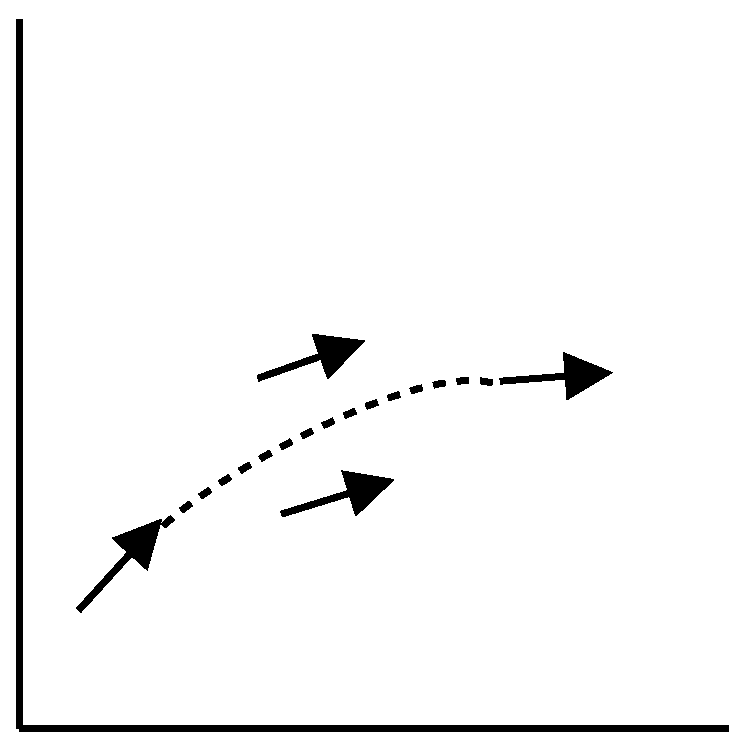
\includegraphics[height=0.25\textheight]{Runge-Kutta}
	\end{center}
    \caption{\label{Fig:Euler}Runge-Kutta method. The diagram shows the
    Runge-Kutta method evaluating the derivative at 4 points, once at the start
    point, once at the endpoint and twice at the midpoints. From this the
    approximation to the function, shown as a dotted line, is calculated.
    This figure is based on the one shown in
    Numerical Recipes \cite{NumRecipes}.}
\end{figure}

\section{Stiffness, Convergence and Stability}
In general a good solver will converge to the solution with the last number of steps.
A solver that diverges, like the Euler method, is in practice not a good choice
for use in computer graphics simulations.
 
\section{Implementation}
\label{DESovlers:sec:Arch}
A further extension is to define the state of the system, $\mathbf{s}$, as 
\[
	\mathbf{s}(t) = 
    \begin{bmatrix}
	    \mathbf{x}(t) \\ 
	    \mathbf{\dot{x}}(t) \\
	\end{bmatrix}
\] 
Therefore the state of the system is a vector of vectors. This contributes to
the final architecture of the numerical differential equation solvers which is
based upon the description given in \cite{PBMNotes}. At the source code level, we
define a class \verb|DEStateSource| that has two essential member functions
\verb|GetState| and \verb|GetStateDerivative|. This class can be used as a base
class to represent any differentiable system, like $e$ or a more complicated
mass spring system. The state of the system $\mathbf{s}(t)$ and its derivative
$\mathbf{\dot{s}}(t)$ are essentially an array of numbers. In the source code
that was written in conjunction with this thesis the state and its derivative is
represented as an array of mathematical vectors.
\lstset{language=C++}
\begin{lstlisting}[basicstyle={\ttfamily \footnotesize}]
class DEStateSource
{
  ....
  void GetState(Array State)
  void GetStateDerivative(Array DState)
  ....
}
\end{lstlisting}
The class \verb|DESolver| has the essential member function \verb|StepState|
that takes the parameters \verb|DEStateSource| and a time delta, $dt$.
\lstset{language=C++}
\begin{lstlisting}[basicstyle={\ttfamily \footnotesize}]
class DESolver
{
  ...
  void StepState(DEStateSource Source, Number dt)
  ...
}
\end{lstlisting}
The implementation of StepState depends on the algorithm used. For example,
below is the pseudo-code for the Euler solver.
\lstset{language=C++}
\begin{lstlisting}[basicstyle={\ttfamily \footnotesize}]
class EulerSolver inherits DESolver
{
  ...
  void StepState(DEStateSource Source, Number dt)
  {
    Array State
    Array DState
    Array NextState
    Source.GetState(State)
    Source.GetStateDerivative(DState)
    for all (s,ds) in (State,DState)
    {
      NextState = s + dt*ds
    }
  }
  ...
}
\end{lstlisting}


